\FloatBarrier
\section{Pore analysis}
\label{sec:pore_analysis}

% pore analysis paper \cite{,levitz.2007,muench.2008,desbois.2016...}

The porosity of a hydrated cement not only defines its final strength, but also its durability, freeze-thaw resistance, and resistance to chemical attack.
On a first glance, the measurement of pores and pore sizes seems to be fairly easy.
However, while air voids in mortar and concrete are mostly spherical due to the surface tension of the fresh binder, this significantly changes below a scale of tens of micrometres, where the capillary porosity begins.
These pores are filled with pore solution/water during hydration and feature much more complex, fractal-like geometries.

There are a variety of methods to measure the \ac{PSD} of a hardened specimen.
However, each method has different measurement ranges as illustrated in \zcref{fig:pore_sizes}.

\begin{figure}[!ht]
	\centering

	\includegraphics[width=\textwidth]{methods/pore_sizes.pdf}
	\caption{
		Visualisation of phase and pore sizes compared to the rough measurement ranges of selected methods.
		Redrawn according to a figure by \textcite{stark.2000}, based on data from \textcite{romberg.1978}.
		Extended by data from \cite{aidukas.2024, wang.2017}.
	} 
	% wang.2017 - NMR 2nm-200µm
	% aidukas.2024 PXCT 4nm - ...
	\label{fig:pore_sizes}
\end{figure}

Image-based methods like \ac{SEM}, \ac{CT}, \ac{PXCT}, and light microscopy are widely used in the cement field for porosity analysis and cover a wide range of scales.
Another lesser known alternative to 3D porosity imaging of cementitious materials is fluorescence \ac{LSCM}.
It allows to record time series of thin specimens \cite{yio.2015a} and can be combined with serial sectioning for volume analysis \cite{yio.2015, yio.2019}. 
However, image-based methods inherently have either a limited resolution, only give a 2D view or do not give representative results due to a small \ac{ROI}.
Therefore, more indirect methods based on physical principles can help to obtain more statistically significant results.
For this work, \ac{MIP} and \ac{LTDSC} were used as complementary methods to the image-based methods.
However, in the literature \ac{HNMR} and \ac{DVS} are also commonly used to characterise the porosity of cementitious materials \cite{naber.2020,pinson.2015}.

% Comparison of pore categories between different authors, from \cite{breugel.1997}, page 77

\subsection{\Acl*{MIP}}
\label{sec:mip}
% \cite{munch.2008} FIB vs MIP!!! (11.9 x10.7 x5.6 µm)
%https://www.epfl.ch/labs/lmc/wp-content/uploads/2019/08/03-Wioletta-Franco-MIP.pdf
\ac{MIP} is a rather old and well-known method, which is used to characterise the \ac{PSD} of a solid material between \qty{3.5}{\nano\meter} to \qty{500}{\micro\meter} by applying pressure to force mercury into the pores \cite{giesche.2002}. % \cite{romberg.1978}
However, the pore size range is a constant point of discussion in the literature and depends on the type of material to be measured. % cite?
Mercury is used due to its non-wetting properties and the high surface tension \cite{giesche.2002}. % of \qty{4850}{\newton\per\meter} 
The fundamental principle is governed by the \textcite{washburn.1921} equation, which relates the applied pressure required to force mercury into a cylindrical pore to the pore's radius, the surface tension of mercury, and the contact angle between mercury and the sample material.
Smaller pores require significantly higher pressures for mercury intrusion.
By precisely measuring the volume of mercury intruded into the sample at each pressure increment, a detailed pore size distribution can be obtained.

In 2024, \textcite{georget.2024} still deemed \ac{MIP} a reliable method, since it delivers a similar volume of capillary porosity (defined as >\,\qty{5}{\nano\meter}) compared to \ac{HNMR}.
According to \textcite{muller.2014}, the \ac{MIP} technique allows adequate quantification of the capillary porosity of hydrated cement as long as it is dried properly using the solvent exchange method.
However, it was seen to be unreliable to extract the porosity of \ac{CSH} as it overestimates the porosity by up to a factor of \num{3} to \num{4} \cite{muller.2014}.
\ac{MIP} is also considered inappropriate by \textcite{diamond.2000} to measure the \ac{PSD} of hydrated cement, since it `\textit{systematically misallocates the sizes of almost all of the volume of pores}', which is agreed upon by others \cite{chatterji.2001,giesche.2002}.
The `ink-bottle' effect (see \zcref{fig:mip-bottle-neck}) is often mentioned as the reason for this misallocation.
\begin{figure}[!ht]
	\centering

	\ifdefined\PRINTABLE
		\includegraphics[width=.95\textwidth]{mip/bottle-neck_6.pdf}
	\else
		\animategraphics[autoplay,poster=6,width=.959\linewidth]{1}{mip/bottle-neck_}{0}{6}
	\fi
	
	\caption{
		Illustration of the ink-bottle effect (not to scale).
		Grey: sample; (a) coloured by pressure: \ce{Hg}; (c) {\color{blue}blue}: \ce{Hg}.
		During the intrusion (a), the pores will be filled from {\color{green}$d_1$} to {\color{orange}$d_3$}, while the small pore diameter {\color{red}$d_4$} (bottle-neck) is blocking the access to the larger pore with the diameter {\color{red}$d_5$}.
		Therefore, the pore volume $V_5$ is measured together with $V_4$ at pressure $p_4$ (c).
		After the depressurisation, mercury will remain trapped within the pores (c, {\color{blue}blue}), causing a hysteresis curve (b).
	}
	\label{fig:mip-bottle-neck}
\end{figure}

\textcite{wang.2019} showed the damage induced by \ac{MIP} using \ac{mCT}.
They came to the conclusion that the pore space was increased by $\approx$ \qty{7}{\percent} due to the mercury intrusion.
The main affected pore size range was around \qtyrange{100}{500}{\micro\meter}.
Furthermore, \ac{MIP} requires dried specimens, leading to cracked and therefore non-native microstructures \cite{chatterji.2001,wang.2019}.

\textcite{abell.1999} and \textcite{hildenbrand.2003} compared \ac{MIP} with the intrusion of \textsc{Wood}'s metal instead of mercury.
In cement, the pore volume was comparable; the usage of \textsc{Wood}'s metal indicated that larger pores were present \cite{abell.1999}.
\textcite{hildenbrand.2003} applied this comparison to mudstones and concluded that \ac{MIP} causes a significant compression of the sample pore space.
This was already assumed by \cite{horseman.1996} who declared \ac{MIP} as `totally unreliable' for clay-like materials.
\textcite{hall.1986} concludes in comparison with small angle neutron scattering and \ce{N2} measurements (e.g. \ac{BET}), that pores larger than \qty{70}{\nano\meter} in clays may be preparation artefacts (e.g. due to drying).
\ac{MIP} was also deemed inadequate for oolitic limestone by \textcite{roels.2001} due to the ink-bottle effect.
They preferred the main wetting curve, \ac{SEM} images, and pressure membrane apparatus measurements of saturated specimens over \ac{MIP}.

Finally, due to the use of hazardous mercury and the high cost, it has a reduced relevance today.
Despite its flaws, \ac{MIP} is useful to compare the porosity of similar samples or the relative change in porosity within a specimen \cite{juntgen.1966}.



%im hinblick auf mögliche gutachterinnen: hast du gecheckt, ich glaube hong wong zusammen mit buenfeld haben sich auch dazu geäußert
% \cite{wong.2006} BSE porosity
% \cite{wong.2012} BSE porosity - Estimating the permeability of cement pastes and mortars using image analysis and effective medium theory



\FloatBarrier
\subsection{\Acl*{LTDSC}}

Another method to indirectly measure the \ac{PSD}, especially in the nanopore range, is \ac{LTDSC} \cite{brun.1973,brun.1977}, often also called \textit{thermoporometry} (e.g. \cite{joseph.2024}).
The method is based on the principle that the freezing point of water is lowered in small pores due to surface tension \cite{brun.1973,brun.1977}.
Since the heat capacity of the phase transition (liquid-solid) is significantly higher than that of the solid phases, this freezing point depression can be measured using \ac{DSC}.

%\qtyrange{2}{3.19}{\nano\meter}
The measurable pore size range starts at approx. \qty{2}{\nano\meter} \cite{cuperus.1992} due to a temperature limit in the thermodynamic description of \qty{-40}{\celsius} \cite{brun.1977}.
However, this limit can be ignored and extended to lower temperatures and smaller pores when considering the extrapolated curve for the triple point depression in porous materials \cite{kloetstra.1995}.
For pores larger than \qty{30}{\nano\meter} the temperature shift of the freezing point is too small to be separated from the freezing of free water \cite{cuperus.1992,stocker.2002}.

\ac{LTDSC} requires water-saturated specimens and therefore avoids damage due to drying \cite{gran.1997,galle.2001} often criticised in \ac{MIP} and \ac{SEM} experiments \cite{chatterji.2001,georget.2024}.
\textcite{sant.2011} applied \ac{LTDSC} to measure the \ac{PSD} of hydrated cement pastes.
They proposed the connection between pore types and the freezing point depression (ranges in brackets are extracted from graphs in \cite{sant.2011}):
\begin{itemize}
	\item connected capillary pores freeze at $\approx$ \qty{-15}{\celsius} (\num{0} to \qty{-23}{\celsius})
	\item open gel pores and capillary pores at $\approx$ \qty{-27}{\celsius} (\num{-23} to \qty{-35}{\celsius})
	\item isolated capillary and gel pores at $\approx$ \qty{-43}{\celsius} (\num{-35} to \qty{-50}{\celsius})
\end{itemize}
In their study, only the peak presence at $\approx$ \qty{-15}{\celsius} was evaluated.

The freezing point of a solution is typically lower than that of the pure solvent.
In cementitious materials, the pores are filled with a saturated \ce{Ca(OH)2} solution.
As calculated in \zcref{sec:freezing-point-depression}, this results in a freezing point of \qty{-0.06}{\celsius}.

\textcite{brun.1977} proposed an approximate solution to convert between freezing/melting point of water and the pore radius for cylindrical pores. %based on a \textsc{Gibbs-Thompson} relationship 
The equation for freezing is:
\begin{equation}
	r_\text{P} = -\frac{\qty{64.67}{\nano\meter\per\kelvin}}{\Delta T }+\qty{0.57}{\nano\meter};~~~\qty{-40}{\kelvin} < \Delta T < \qty{0}{\kelvin},
	\label{eq:brun_freeze}
\end{equation}
\begin{conditions}
	r_\text{P} & pore radius in \unit{\nano\meter}\\
	\Delta T  &  freezing point depression in \unit{\kelvin},
\end{conditions}

and for melting:
\begin{equation}
	r_\text{P} = -\frac{\qty{32.33}{\nano\meter\per\kelvin}}{\Delta T }+\qty{0.68}{\nano\meter};~~~\qty{-40}{\kelvin} < \Delta T < \qty{0}{\kelvin}.
	\label{eq:brun_melt}
\end{equation}
% in Joseph.2024 stammt die + 0.68 aus "-0.12 + \delta" wobei \delta = the non-freezable layer of water in nm. With respect to the value of δ, both 1.2 nm [52,53] and 0.8 nm [51,54]

$\Delta T$ is defined as:

\begin{equation}
	\Delta T = T - T_\text{m}
	\label{eq:brun_dT}
\end{equation}
\begin{conditions}
	T          &   actual melting point in \unit{\kelvin}, \\
	T_\text{m} &   theoretical freezing point in \unit{\kelvin}.
\end{conditions}

It has to be noted that \textcite{brun.1977} experimental investigations of water, from which these numerical approximations were derived, were limited to a temperature range of $\qty{-40}{\kelvin} < \Delta T < \qty{0}{\kelvin}$.
Therefore, the equations lack validation for freezing point depressions below \qty{-40}{\celsius}.
However, \textcite{kloetstra.1995} applied these relations to their mesoporous materials and noted that the extrapolated curve for the triple point depression in porous materials shows that the relations can also be used at lower temperatures.

%\begin{wrapfigure}{R}{0.6\linewidth}
\begin{figure}[!htb]
    \centering
	%\vspace{-\intextsep}
    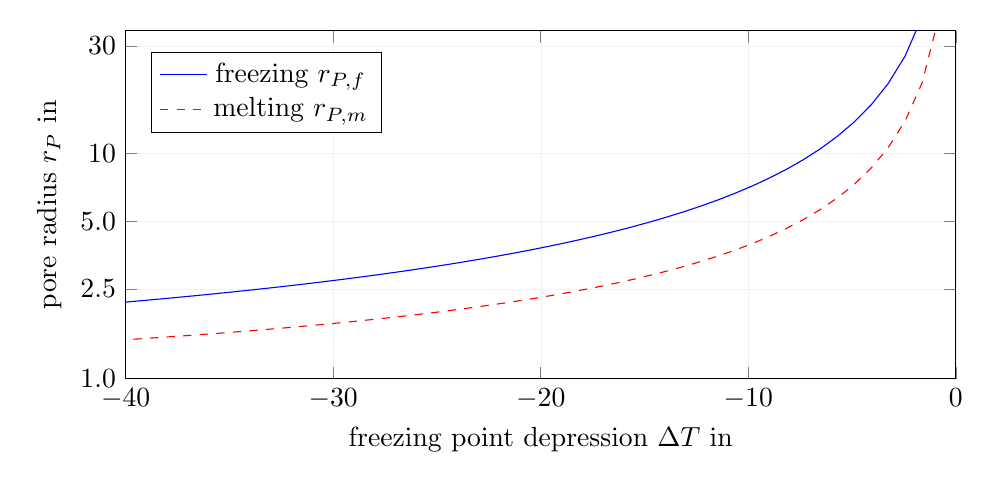
\begin{tikzpicture}
        \begin{semilogyaxis}[
				legend style={at={(0.03,.94)},anchor=north west},
				xmin=-40, xmax=0,
				ymin=1, ymax=35,
				width=\linewidth,
				height=6cm,
				grid=major,
				xlabel={freezing point depression $\Delta T$ in \unit{\kelvin}},
				ylabel={pore radius $r_\text{P}$ in \unit{\nano\meter}},
				xtick={0,-10,...,-40},
				ytick     ={1,2.5,5,10,30},
				yticklabels={1.0,2.5,5.0,10,30},
				grid style={line width=.1pt, draw=gray!10},
				%x dir=reverse
            ]
			\addplot[blue, domain=0:-40, samples=50] {0.57-64.67/x};
            \addlegendentry{freezing $r_\text{P,f}$};
			\addplot[red, domain=0:-40, samples=50, dashed] {0.68-32.33/x};
            \addlegendentry{melting $r_\text{P,m}$};
        \end{semilogyaxis}
    \end{tikzpicture}
    \caption{
		Depression of the freezing or melting point as functions of the pore radius.
		Calculated according to \textcite{brun.1977} for water using \zcref{eq:brun_freeze, eq:brun_melt}.
		The pore radius $r_\text{P}$ is plotted logarithmically.
	}
	%\vspace{-\intextsep}
    \label{fig:freezing_depression}
\end{figure}
%\end{wrapfigure}
% TODO: Stockhausen??

\textcite{brun.1977} considered an adsorbed water film in the pores (thickness of \qty{0.8}{\nano\meter}) and also a temperature correction for surface tension and for the melting entropy.
The correlations resulting from \zcref{eq:brun_freeze, eq:brun_melt} are plotted in \zcref{fig:freezing_depression}.
This shows that smaller pores lead to lower freezing temperatures of the water inside the pores.
However, this also depends on the pore type.


%\begin{wrapfigure}{R}{0.5\textwidth}
\begin{figure}[!htb]
    \centering
	%\vspace{-\intextsep}
	\ifdefined\PRINTABLE
		\includegraphics[width=.5\linewidth]{ltdsc/ltdsc_freezing3.pdf}
	\else
		\animategraphics[loop,poster=last,autoplay,width=.5\linewidth]{1}{ltdsc/ltdsc_freezing}{0}{3}
	\fi

    \caption{
		Scheme of the freezing process within a connected pore system.
		Freezing happens sequentially from $d_1$ to $d_2$, followed by $d_3$ and $d_4$ at once. Based on \textcite{sun.2010}.
	}
	%\vspace{-\intextsep}
    \label{fig:freeze}
\end{figure}
%\end{wrapfigure}

If a larger pore ($d_4$) is only connected to smaller pores ($d_3$) or is isolated, it can only freeze at the same temperature as the smaller pores ($d_3$), while pores with a similar size ($d_2$) were already frozen (\zcref{fig:freeze}).

Furthermore, supercooling effects can be observed in the literature \cite{setzer.1994,sant.2011}, which renders the evaluation of the larger pore sizes more difficult or impossible.
They are indicated by a shift of the main freezing peak to temperatures below \qty{-10}{\celsius}.
The reason for the supercooling is the lack of nucleation points for the ice crystals.
Therefore, in more recent publications a pre-cooling step was carried out to induce nucleation crystals \cite{nguyen.2021,mueller.2021,joseph.2024}.

This raises the question of whether the pore structure will be damaged as observed in \ac{MIP}.
\Textcite{wu.2015} concluded that the heat flow curves were not affected by a preceding freeze cycle and there is little impact on the pore structure for porous silica.
They also applied the method to cementitious samples and detected the expected peak shift for connected capillary pores (above \qty{-40}{\celsius}).
However, a signal change in the isolated gel porosity (below \qty{-40}{\celsius}) was also noticed.
It was assumed that the pore connectivity changed between the measurements.
This was indicated by a signal shift in the direction of higher freezing temperatures and therefore larger pores.
%, while having limited effect on the size distribution of mesopores.

\Textcite{neffati.2001} studied the influence of the heating rate on the \ac{LTDSC} results using porous glass.
They found that slower heating rates lead to narrower peaks and a lower signal response.
Heating rates of more than \qty{2}{\kelvin\per\minute} were considered too imprecise to study the pore size distribution.
However, cooling/heating rates below \qty{0.1}{\kelvin\per\minute} were considered to have a poor signal-to-noise ratio.
While \textcite{joseph.2024} used \qty{0.5}{\kelvin\per\minute} as a compromise, \textcite{wu.2015} and \textcite{ghantous.2023} still used a cooling/heating rate of \qty{0.1}{\kelvin\per\minute} to measure the porosity of cementitious materials.
%{\color{red}Considering the higher sensitivity of more modern devices, this heating rate could still be valid.}
%10.14359/51738808 \cite{Ghantous.2023} Examining Effect of Printing Directionality on Freezing and-Thawing Response of Three-Dimensional-Printed Cement Paste

\subsection{Further non-image-based methods}
\label{subsec:other_porosity}

Other methods to obtain information about the porosity of materials are based on their respective response to the diffusion, permeability or the sorption of various gases like \ce{N2}, \ce{O2} or water vapour.
Furthermore, \ac{HNMR} can be used to measure the porosity of a material.

\subsubsection[Proton nuclear magnetic resonance spectroscopy]{\Acl*{HNMR}}

\ac{HNMR} can be used to evaluate the porosity of cementitious materials at room temperature without the need for drying or freezing, which would change its microstructure \cite{gran.1997,muller.2014,naber.2020}.
It is based on the magnetic resonance of the \ce{^1H} nuclei, primarily found in water molecules.
The method involves placing a water-saturated sample in a strong magnetic field and perturbing the hydrogen nuclei spins with magnetic pulses.
The subsequent relaxation of these nuclei back to their equilibrium state generates a measurable signal.
The key principle is that the \ac{NMR} relaxation time (particularly the transverse relaxation time, $T2$) of water molecules confined within pores is significantly affected by their interaction with the pore surfaces. % hier muss ich mich nochmal einlesen
However, this method is not suitable for materials with a significant content of paramagnetic species (like iron oxides) \cite{barrie.2000}. 
These species alter the relaxation behaviour of the protons, thereby interfering with the measurement \cite{muller.2014}.

\ac{NMR} allows the analysis of the porosity of a specimen in a wide range, including porosity below \qty{2}{\nano\meter} \cite{barrie.2000}. 
Therefore, it is especially useful to gain insight into the interlayer volume of the \ac{CSH} phases.
For example, \textcite{naber.2020} combined \ac{SEM} image analysis with \ac{HNMR} relaxometry.
They used high-resolution \ac{SEM} images of \ac{ArBIB}-milled surfaces to determine the surface-to-volume ratio of the larger interhydrate pores, which are mostly unaffected by sample preparation.
This geometrical data was then used to calibrate the surface relaxivity parameter for the \ac{HNMR} measurements.
Consequently, they were able to calculate the sizes of the nanoscale gel and interlayer pores from the \ac{HNMR} data without relying on theoretical assumptions about water monolayer coverage.
%W. P. Halperin, J.-Y. Jehng, Y.-Q. Song, Application of spin-spin relaxation to measurement of surface area and pore size distributions in a hydrating cement paste, Magnetic  Resonance Imaging 12 (2) (1994) 169–173.#

\subsubsection[Dynamic vapour sorption]{\Acl*{DVS}}

\Ac{DVS} can give a rough idea of the porosity of a material \cite{pinson.2015} and the behaviour of the material under changing humidity at different temperatures \cite{wang.2023}.
While the operating gas is variable, it is usually water.

The method works by placing a dry specimen in a humidity-controlled chamber, while stepwise increasing the humidity and measuring the mass change of the specimen until mass consistency is reached.
This is followed by a subsequent stepwise reduction of the humidity.
Depending on the available and accessible pore classes (capillary or gel porosity), the amount of mass change can indicate their presence at different humidities during the drying step \cite{pinson.2015}.
Depending on the device used and the experimental setup, the measurements can take multiple days or weeks at or below room temperature \cite{wang.2023}.

Therefore, this method is only useful for fully hydrated specimens.
For specimens younger than \qty{14}{\day}, this method is not suitable, since hydration can continue significantly during the measurement period.
Furthermore, most authors do not directly evaluate the porosity of the specimen using this method but use it comparatively between specimens or parameters \cite{ghantous.2023, wang.2023}.

\subsection{Comparison-studies of pore analysis methods}
\label{subsec:pore_comparison}

Given the different physical principles and measurement ranges of the various pore analysis methods, multiple studies have attempted to compare their results \cite{munch.2008, naber.2020, georget.2024}.
Since each technique requires specific sample preparation and probes different aspects of the pore network, direct comparisons are often difficult or impossible.

To explain the frequently observed discrepancies between image-based methods and \ac{MIP}, \textcite{munch.2008} compared \ac{MIP} measurements with simulated intrusion algorithms applied to a \ac{FIBnt} 3D volume (\qtyproduct{11.9 x 10.7 x 5.6}{\micro\meter\cubed}).
While standard image analysis typically determines a `discrete' \ac{PSD} by assigning a single equivalent radius to each separated pore object, \ac{MIP} inherently measures a `continuous' \ac{PSD} by decomposing interconnected pore networks into a continuous size spectrum.
This indicates that while the ink-bottle effect still plays a significant role in underestimating larger pores in a \ac{MIP} analysis, the geometric definition of a pore size is the main reason for deviations between microscopy and intrusion techniques.

To overcome the ink-bottle effect and to validate \ac{mCT} and \ac{SEM} measurements, alternative intrusion techniques have been explored.
\textcite{qian.2018} utilised a metal alloy with a melting of \qty{47}{\celsius} to intrude the pore space by centrifugation.
By analysing the metal distribution using \ac{SEM} and \ac{mCT}, they achieved a high-contrast 3D visualisation of the pore structure.
Compared to \ac{MIP}, the total porosities were consistent, but the metal intrusion revealed larger most-probable pore sizes.
This directly demonstrated the underestimation caused by the ink-bottle effect and sectioning differences in \ac{MIP}.

\textcite{georget.2024} systematically compared \ac{MIP}, \ce{N2}-adsorption, \ac{HNMR}, and \ac{SEM} image analysis.
They highlighted that only methods measuring liquid water (such as \ac{HNMR}) can reliably access the true gel porosity.
The drying steps necessary for \ac{MIP} and \ce{N2}-adsorption inevitably lead to a partial change of the gel porosity, shifting these pore sizes towards the capillary pore range.
Furthermore, they concluded, that the evaluation of only a single segmented \ac{SEM}-\ac{BSE} image ($\approx$ \qty{0.3}{\milli\meter\squared} at $\approx$ \qty{0.1}{\micro\meter\per\px}) per specimen is not sufficient for a reliable pore analysis.

% Note: joseph.2024 also indicates that a cooling rate of 0.5 K/min might be more appropriate than 2 K/min to avoid shifting pore sizes to smaller values.
Comparisons between \ac{MIP} and \ac{HNMR} can be complicated, and their respective \ac{PSD}s often do not fit perfectly \cite{tziotziou.2011}.
This discrepancy arises primarily because \ac{MIP} measures the distribution of pore throats, whereas \ac{HNMR} surveys the actual pore body dimensions based on the enclosed water volume.
\textcite{joseph.2024} also compared \ac{HNMR}, \ac{MIP}, and \ac{LTDSC}.
They found, considerable deviations for pores larger than \qty{10}{\nano\meter} in mature pastes using \ac{MIP}, which was attributed to the required drying processes.
They concluded that while \ac{HNMR} and \ac{LTDSC} yield similar \ac{PSD}s for saturated pores, \ac{HNMR} provides more comprehensive data for pores smaller than \qty{3}{\nano\meter}, as \ac{LTDSC} cannot fully capture the non-freezable water layers.
